%%%%%%%%%%%%%%%%%%%%%%%%%%%%%%%%%%%%%%%%%%%%%%%%%%%%%%%%%%%%%%%%%%%%%%%%%%%%%%%%%%%%%%%
%%%%%%%%%%%%%%%%%%%%%%%%%%%%%%%%%%%%%%%%%%%%%%%%%%%%%%%%%%%%%%%%%%%%%%%%%%%%%%%%%%%%%%%
% 
% This top part of the document is called the 'preamble'.  Modify it with caution!
%
% The real document starts below where it says 'The main document starts here'.

\documentclass[12pt]{article}

\usepackage{amssymb,amsmath,amsthm}
\usepackage[top=1in, bottom=1in, left=1.25in, right=1.25in]{geometry}
\usepackage{fancyhdr}
\usepackage{enumerate}
\usepackage{listings}
\usepackage{graphicx}
\usepackage{float}
\usepackage{multirow}

\usepackage{mwe}
\usepackage{caption}
\usepackage{subcaption}
% Comment the following line to use TeX's default font of Computer Modern.
\usepackage{times,txfonts}



\makeatletter
\renewcommand*\env@matrix[1][*\c@MaxMatrixCols c]{%
  \hskip -\arraycolsep
  \let\@ifnextchar\new@ifnextchar
  \array{#1}}
\makeatother

\newtheoremstyle{homework}% name of the style to be used
  {18pt}% measure of space to leave above the theorem. E.g.: 3pt
  {12pt}% measure of space to leave below the theorem. E.g.: 3pt
  {}% name of font to use in the body of the theorem
  {}% measure of space to indent
  {\bfseries}% name of head font
  {:}% punctuation between head and body
  {2ex}% space after theorem head; " " = normal interword space
  {}% Manually specify head
\theoremstyle{homework} 

% Set up an Exercise environment and a Solution label.
\newtheorem*{exercisecore}{Exercise \@currentlabel}
\newenvironment{exercise}[1]
{\def\@currentlabel{#1}\exercisecore}
{\endexercisecore}

\newcommand{\localhead}[1]{\par\smallskip\noindent\textbf{#1}\nobreak\\}%
\newcommand\solution{\localhead{Solution:}}

%%%%%%%%%%%%%%%%%%%%%%%%%%%%%%%%%%%%%%%%%%%%%%%%%%%%%%%%%%%%%%%%%%%%%%%%
%
% Stuff for getting the name/document date/title across the header
\makeatletter
\RequirePackage{fancyhdr}
\pagestyle{fancy}
\fancyfoot[C]{\ifnum \value{page} > 1\relax\thepage\fi}
\fancyhead[L]{\ifx\@doclabel\@empty\else\@doclabel\fi}
\fancyhead[C]{\ifx\@docdate\@empty\else\@docdate\fi}
\fancyhead[R]{\ifx\@docauthor\@empty\else\@docauthor\fi}
\headheight 15pt

\def\doclabel#1{\gdef\@doclabel{#1}}
\doclabel{Use {\tt\textbackslash doclabel\{MY LABEL\}}.}
\def\docdate#1{\gdef\@docdate{#1}}
\docdate{Use {\tt\textbackslash docdate\{MY DATE\}}.}
\def\docauthor#1{\gdef\@docauthor{#1}}
\docauthor{Use {\tt\textbackslash docauthor\{MY NAME\}}.}
\makeatother

% Shortcuts for blackboard bold number sets (reals, integers, etc.)
\newcommand{\Reals}{\ensuremath{\mathbb R}}
\newcommand{\Nats}{\ensuremath{\mathbb N}}
\newcommand{\Ints}{\ensuremath{\mathbb Z}}
\newcommand{\Rats}{\ensuremath{\mathbb Q}}
\newcommand{\Cplx}{\ensuremath{\mathbb C}}
%% Some equivalents that some people may prefer.
\let\RR\Reals
\let\NN\Nats
\let\II\Ints
\let\CC\Cplx
%%%%%%%%%%%%%%%%%%%%%%%%%%%%%%%%%%%%%%%%%%%%%%%%%%%%%%%%%%%%%%%%%%%%%%%%%%%%%%%%%%%%%%%
%%%%%%%%%%%%%%%%%%%%%%%%%%%%%%%%%%%%%%%%%%%%%%%%%%%%%%%%%%%%%%%%%%%%%%%%%%%%%%%%%%%%%%%
% 
% The main document start here.

% The following commands set up the material that appears in the header.
\doclabel{Stat 605: Homework 5}
\docauthor{Stefano Fochesatto}
\docdate{\today}


\begin{document}

\begin{exercise}{1}Use R to plot two Matern semi-variograms on the same graph, one with smoothness parameter
  $v = k = 1/2$, another with $v = k = 5$; in each case use range parameter $a = \phi = 1$. Use a nugget 
  $\tau^2 = 1.0$ and a partial sill of $\sigma^2 = 1.5$. Which of the two semi-variograms corresponds to smoother realizations, 
  and how can you tell?\\
  \solution Firstly we must convert the values from the matern function which calculates a co-variogram into our desired semi-variogram. Recall the
  the relationship between the two variograms, 
  \begin{equation*}
    \gamma(h) = C(0) - C(h),
  \end{equation*} 
  where we think of $C(0)$ as the sill. Since we want a nugget of $\tau^2 = 1.0$ and a partial sill of $\sigma^2 = 1.5$, the function we will use to plot the semivariograms looks like this, 
  \begin{equation*}
    curve((\sigma^2 - \text{matern}(x, \phi, \kappa)) + \tau^2, \text{from} = 0, \text{to} = \text{upperbound}). 
  \end{equation*}
  Plotting the two Matern semi-variograms we get the following, \\
  \textbf{Code:}
  \begin{center}
  \lstinputlisting[basicstyle = \footnotesize]{r1.txt}
  \end{center}
  \begin{figure}[H]
    \begin{center}
    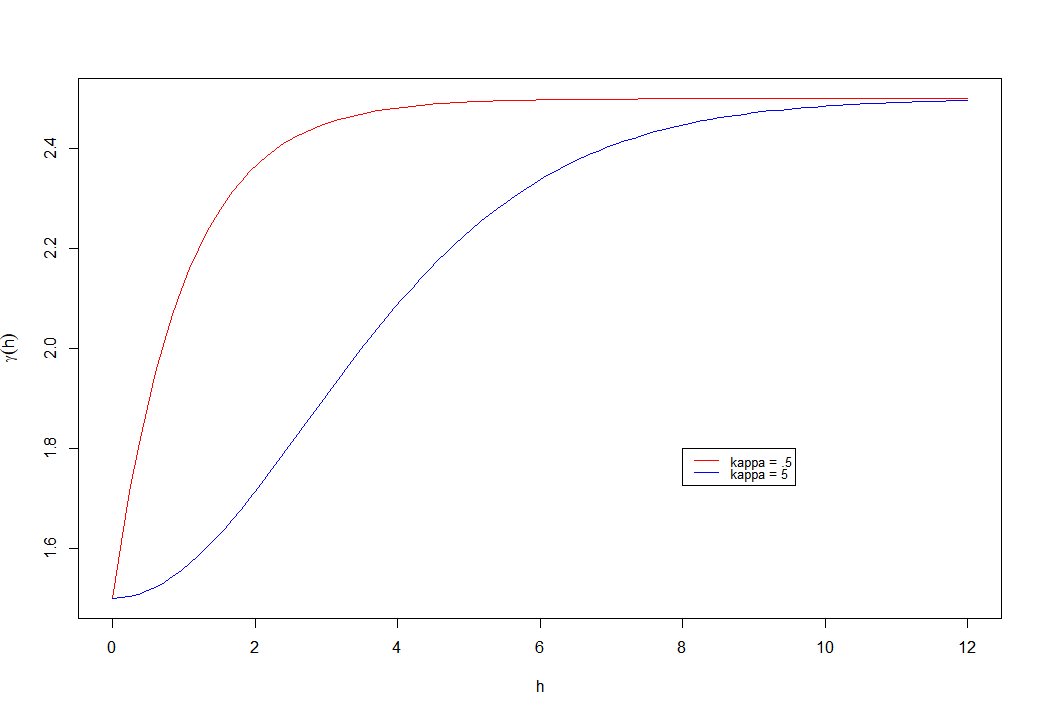
\includegraphics[width = .90\textwidth]{Rplot.png}
    \end{center}
  \end{figure}
  The goal of any covariogram is to quantify the similarity (or difference) between observations as a function of distance. Comparing the two Matern semi-variograms we find that 
  the one with $\kappa = .5$ has a smaller range than the one with $\kappa = 5$. Interpreting this we see that the rate at which observations become significantly different as a function of time
  is greater when $\kappa = .5$. Naturally this leads to a more uneven, discrete looking realization.
\end{exercise}
\vspace{1in}




\begin{exercise}{2} Continuing analysis using R fo the scallop data set using centered lats longs.
  
  \begin{enumerate}
    \item[a] Add borders to the data set that has centered latitudes and longitudes.
    \solution Reading in the data and adding borders using my own add borders function() we get the following, \\
        \textbf{Code:}
      \begin{center}
      \lstinputlisting[basicstyle = \footnotesize]{r2.txt}
      \end{center}
      \begin{figure}[H]
        \begin{center}
          \caption{Plot of scallops geoR object with new borders.}
        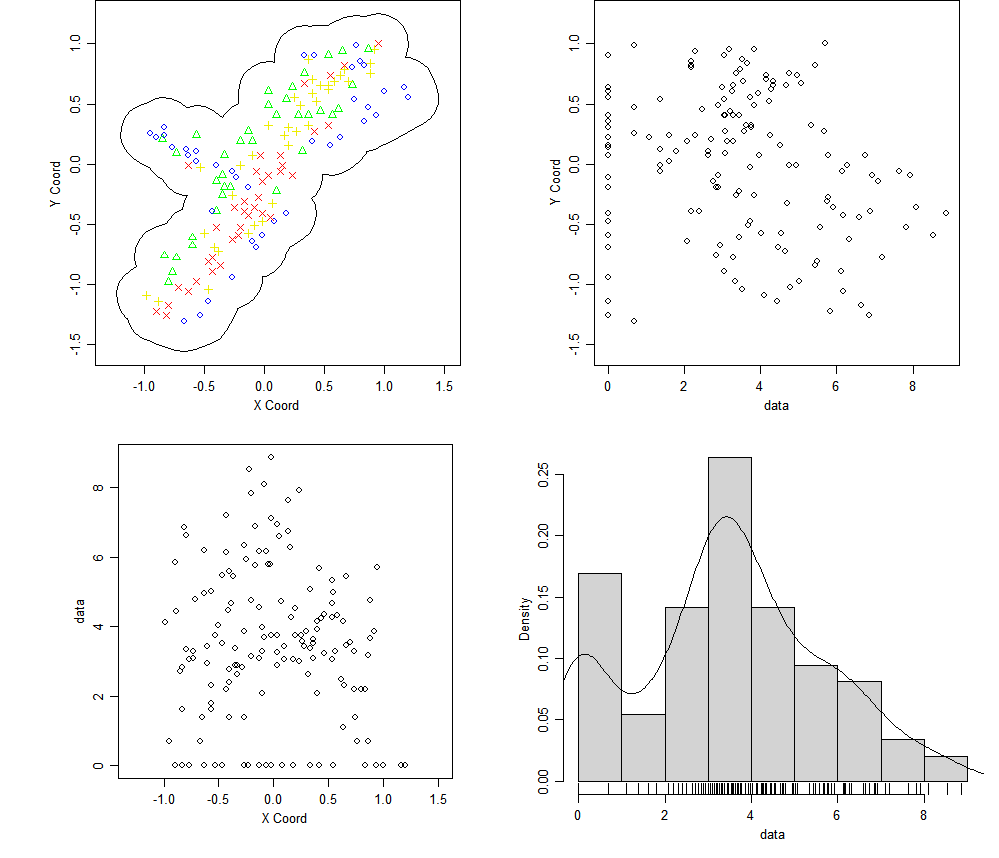
\includegraphics[width = .75\textwidth]{Rplot01.png}
        \end{center}
      \end{figure}

      \vspace{.15in}
   
    \item[b] Use the pred\_grid function to create a suitable grid of prediction locations (using range 
    of values for the centered latitudes and longitudes).\\ 
    \solution We get the range over the centered latitudes and longitudes, then divide it by 100 to fined the necessary spacing, for 
    at least a 100 x 100 resolution. \\
    \textbf{Code:}
    \begin{center}
    \lstinputlisting[basicstyle = \footnotesize]{r3.txt}
    \end{center}
    \vspace{.15in}




    \item[c] Use the krige.control function followed by krige.conv to carry out universal kriging for log(catch)
    at the prediction locations in (b). The R code on pages 96 and 97 may be helpful, as they show you how to handle non-constant trend. 
    You'll probably just need trend.d = '2nd', trend.1 = 'cte' rather than the additional codes in the notes.\\
    \solution Recalling the previous analysis on the scallop data where we computed several estimators for the variogram. I recall that 
    in my analysis a 2nd order gaussian model seemed to fit the best, with the WLS and ML estimators being relatively similar. For this problem 
    I will use the ML estimator, with $\sigma^2 = 3.60472588$, $\phi = .13487626$, and $\tau^2 = .03058721$. Consider the following code,\\
    \textbf{Code:}
    \begin{center}
    \lstinputlisting[basicstyle = \footnotesize]{r4.txt}
    \end{center}
    \vspace{.15in}

    
    \item[d] State the estimated regression equation, $\mathbb{E}(Y(s)) = $?\\
    \solution We can pull the regression coefficients from the my\_kr\_results object. Doing so we get the following, 
    \begin{equation*}
      \mathbb{E}(Y(s)) = 4.161 + (-2.729)lons + (0.727)lats + (-4.406)lons^2 + (-7.153)lats^2 + (11.765)lonslats 
    \end{equation*} 
    \vspace{.15in}




    \item[e] Plot the resulting smoothed map using the centered coordinates.\\
    \solution Using the given one\_plot() function we get the following plot.\\
    \textbf{Code:}
    \begin{center}
    \lstinputlisting[basicstyle = \footnotesize]{r5.txt}
    \end{center}
    \begin{figure}[H]
      \begin{center}
      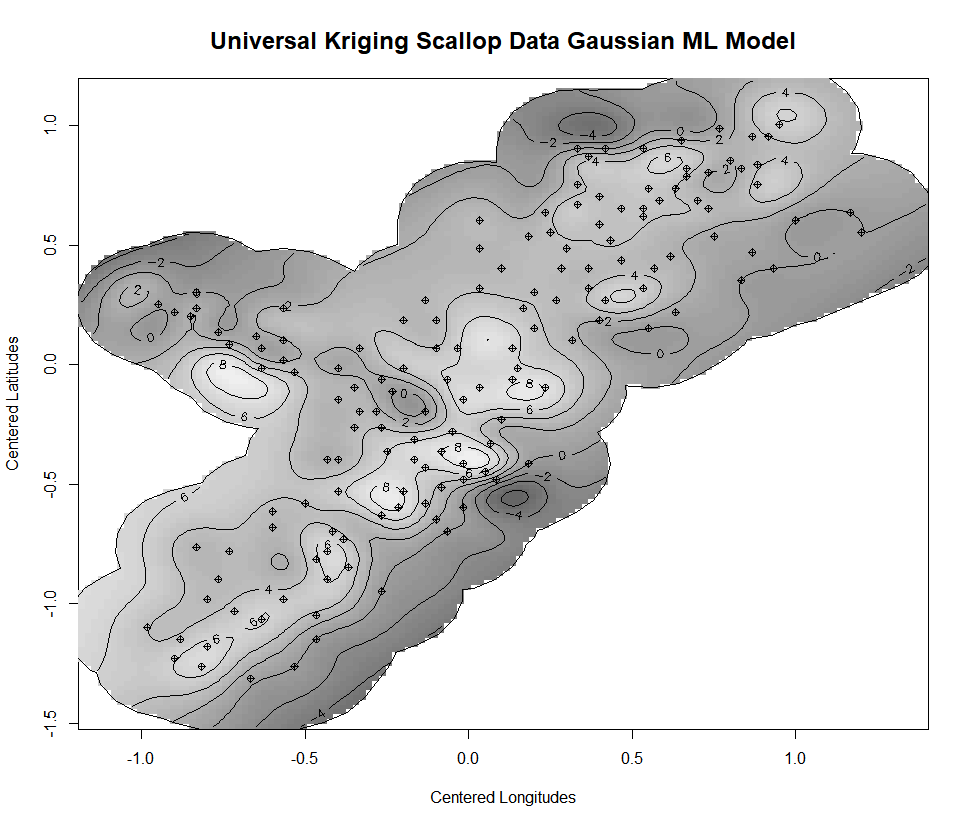
\includegraphics[width = \textwidth]{Rplot02.png}
      \end{center}
    \end{figure}
    \vspace{.15in}

    \item[f] Create a linear interpolation plot of log(catch) using the interp() function in the akima package.
    \solution\\
    \textbf{Code:}
    \begin{center}
    \lstinputlisting[basicstyle = \footnotesize]{r6.txt}
    \end{center}
    \begin{figure}[H]
      \begin{center}
      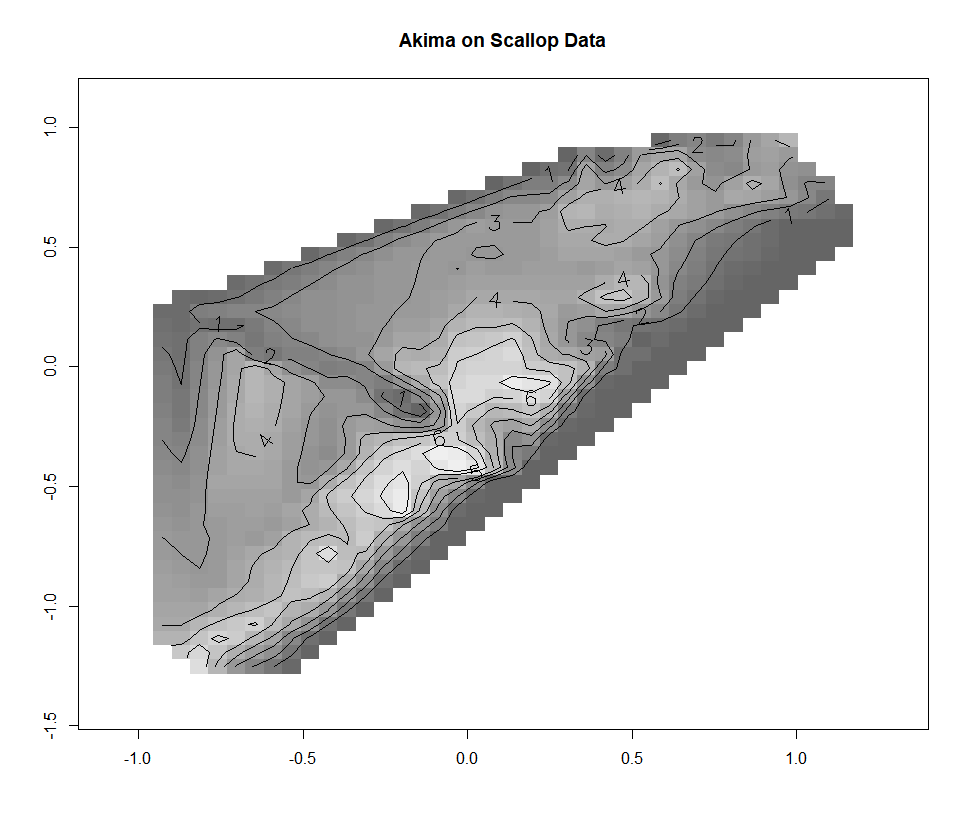
\includegraphics[width = \textwidth]{Rplot03.png}
      \end{center}
    \end{figure}
    \vspace{.15in}

    \item[g] Comment briefly on your result in (e) and (f). (Are the plots the same? Are there any noticeable differences?)
    \solution When we create a linear interpolation of the data, the we can only get a certain amount of smoothness which is predicated on the 
    number of samples, and their proximity. The kriging plot does a better job at creating a smooth map. Beyond that consider the area around point 
    6 from the (f) plot. We can see that in the kriging plot we can see that this area isn't nearly as dark and it has to do with the two 'humps' in the data 
    that are next to it influencing the prediction at that point.  

  \end{enumerate} 
\end{exercise}
\vspace{1in}




\begin{exercise}{3} Kriging weights. Use the spherical semi-variogram model with sill = 4.0, range = 2.0, and nugget = 0 for the following locations:
  \begin{center}
    \begin{tabular}{c|| c c c c c c }
      longitude & 0 & 0 & 1 & 1 & 1.1 & 0.9\\
      \hline 
      latitude & 0 & 1 & 1 & 0 & -0.1 & -0.1\\
     \end{tabular}
    \end{center}

  Construct a plot for these locations and calculate the kriging weights at each of the following five locations, $s_0$
  \begin{center}
  \begin{tabular}{c|| c c c c c c }
    longitude & .5 & .01 & .25 & 1.1 & 1.05\\
    \hline 
    latitude & .5 & .9 & .75 & -0.1 & -0.05\\
   \end{tabular}
  \end{center}
  In each case, comment on the weights, using your plot to assist in your description. For example, for each $s_0$, which observation locations have the largest 
  weights, and does this make sense?\\
  \solution First we begin by creating our kriging object with the desired spherical semi-variogram using krig.control(), then plotting our given locations, \\
  \textbf{Code:}
  \begin{center}
  \lstinputlisting[basicstyle = \footnotesize]{r7.txt}
  \end{center}
  \begin{figure}[H]
    \begin{center}
    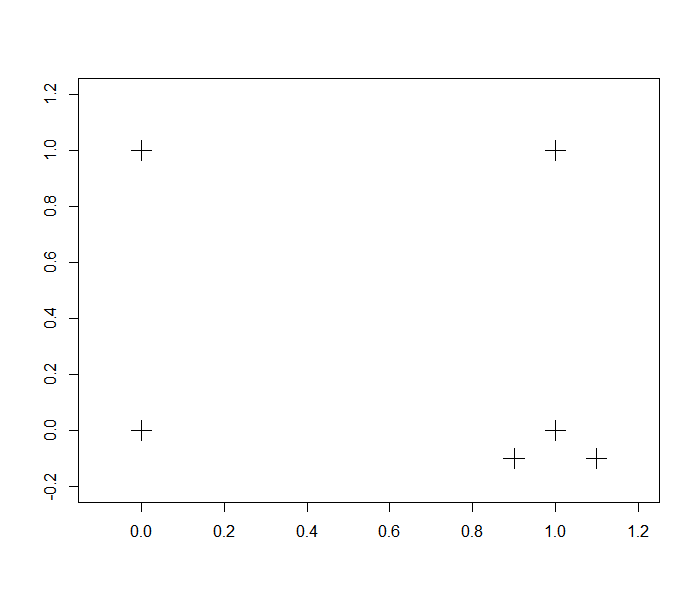
\includegraphics[width = \textwidth]{Rplot04.png}
    \end{center}
  \end{figure}

  Computing the kriging weights for (.5, .5) we get the following with the order corresponding to our initial table. 
  \begin{equation*}
    [0.237 ,0.251,  0.254,  0.267, -0.149,  0.139]
  \end{equation*}
  \textbf{Code:}
  \begin{center}
  \lstinputlisting[basicstyle = \footnotesize]{r8.txt}
  \end{center}
  \begin{figure}[H]
    \begin{center}
    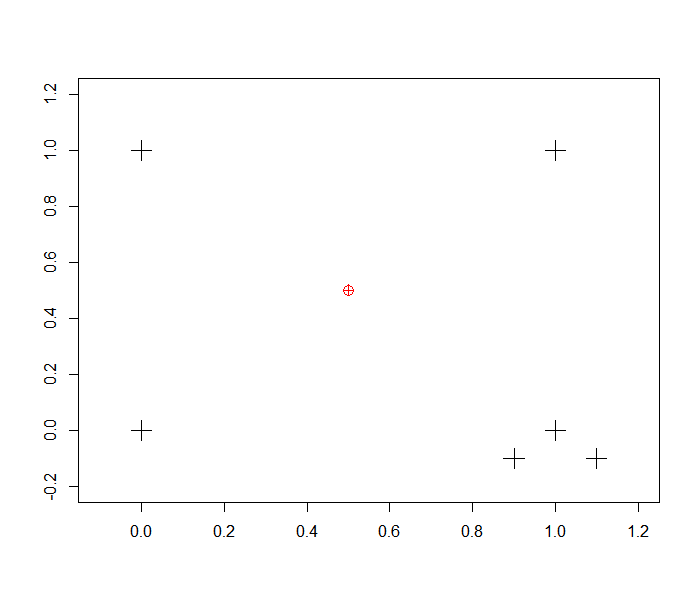
\includegraphics[width = \textwidth]{Rplot05.png}
    \end{center}
  \end{figure}
  This makes sense, looking at the plot the point (.5, .5) is really in the middle of the plot with the first four locations being 
  equidistant from the (.5, .5) point, and the last cancelling each other out.  \\

  Computing the kriging weights for (.1, .9) we get the following with the order corresponding to our initial table. 
  \begin{equation*}
    [0.0793 ,  0.8280,  0.0811, 0.0420, -0.0440, 0.0140]
  \end{equation*}
  \textbf{Code:}
  \begin{center}
  \lstinputlisting[basicstyle = \footnotesize]{r9.txt}
  \end{center}
  \begin{figure}[H]
    \begin{center}
    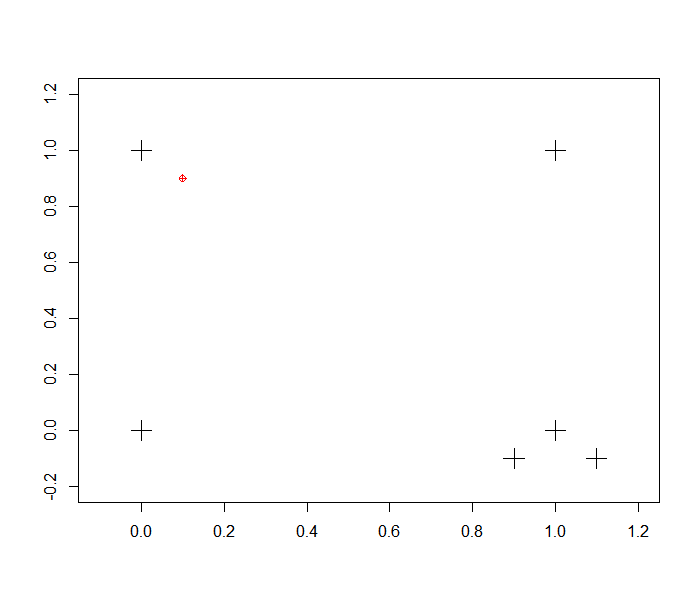
\includegraphics[width = \textwidth]{Rplot06.png}
    \end{center}
  \end{figure}

  Given that  (.1, .9) is closest to (0 , 1) it makes sense that the second weight is the largest. We also see that the first and third weights 
  are relatively the same since they correspond to the (0,0) and (1,1) respectively. The fourth and fifth weight cancel each other out and the last weight 
  sort of makes up for the difference between the first and third.   \\


  Computing the kriging weights for (.25, .75) we get the following with the order corresponding to our initial table. 
  \begin{equation*}
    [0.1750,  0.5820,  0.1810,  0.1130, -0.0969,  0.0462]
  \end{equation*}
  \textbf{Code:}
  \begin{center}
  \lstinputlisting[basicstyle = \footnotesize]{r10.txt}
  \end{center}
  \begin{figure}[H]
    \begin{center}
    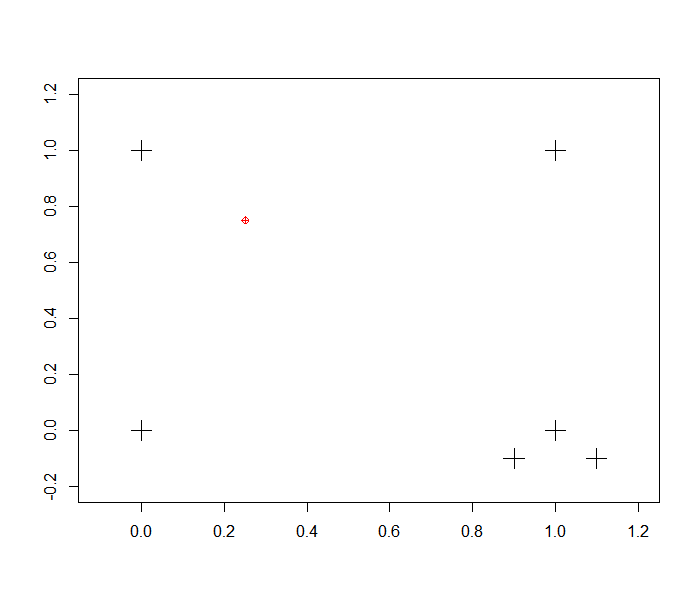
\includegraphics[width = \textwidth]{Rplot07.png}
    \end{center}
  \end{figure}
  This point results in similar weight to the last point with the second weight being a little smaller and the rest of them generally increasing. We still have the fourth and 
  fifth weight, however I imagine the weight of the three locations in the lower right is increased from the last point.\\




  Computing the kriging weights for (1.1, -.01) we get the following with the order corresponding to our initial table. 
  \begin{equation*}
    [-0.006830, -0.000545,  0.034600,  0.501000,  0.555000, -0.083900]
  \end{equation*}
  \textbf{Code:}
  \begin{center}
  \lstinputlisting[basicstyle = \footnotesize]{r11.txt}
  \end{center}
  \begin{figure}[H]
    \begin{center}
    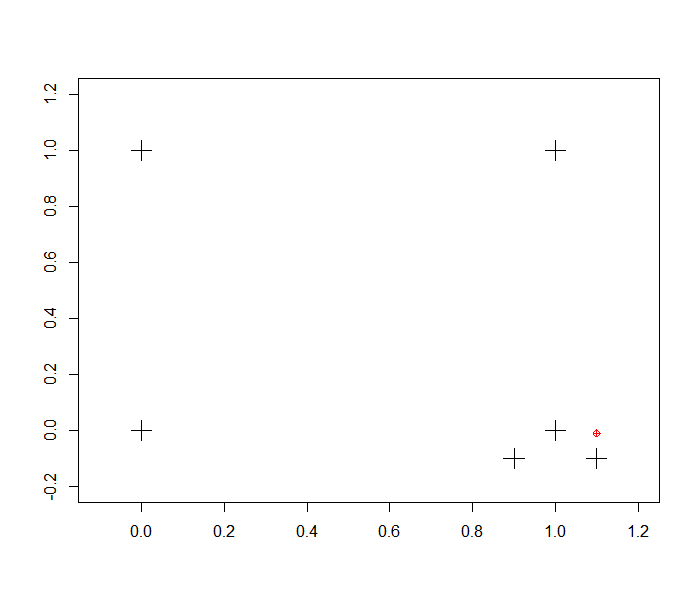
\includegraphics[width = \textwidth]{Rplot08.png}
    \end{center}
  \end{figure}
  Given that (1.1, -.01) is nearest to the three locations in the lower right corner it makes sense that all other weights should be 
  very small. It seems as though weight 3 and specifically 6 might be cancelling each other out with the rest of the influence from the three grouped 
  locations being spread between weight 4 and 5.\\





  Computing the kriging weights for (1.05, -.05) we get the following with the order corresponding to our initial table. 
  \begin{equation*}
    [-0.00514, -0.00158,  0.00155,  0.46600,  0.48600,  0.05300]
  \end{equation*}
  \textbf{Code:}
  \begin{center}
  \lstinputlisting[basicstyle = \footnotesize]{r11.txt}
  \end{center}
  \begin{figure}[H]
    \begin{center}
    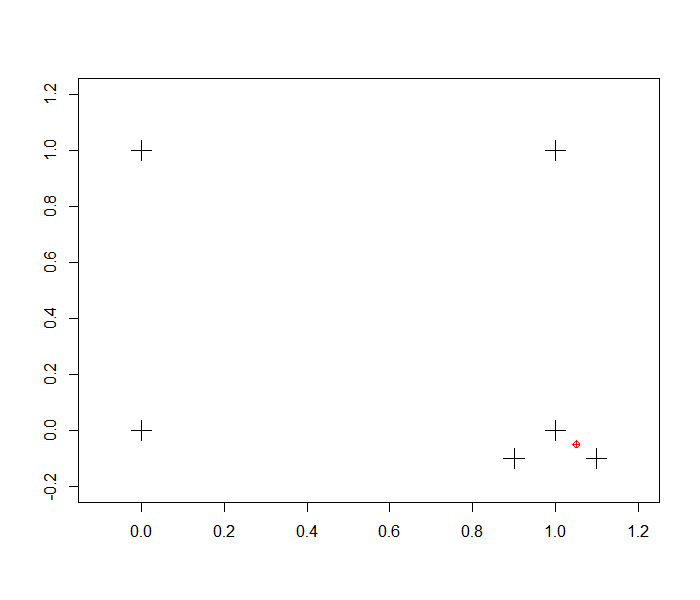
\includegraphics[width = \textwidth]{Rplot09.png}
    \end{center}
  \end{figure}
  Again we have a similar situation as before with the point (1.05, -.05) being really close to the three location in the lower right.





  
  










  
  







\end{exercise}






\end{document}

